\chapter{Proposta deste projeto}

Neste capítulo pretende-se apresentar a proposta de uma arquitetura que visa sustentar o desenvolvimento de aplicações de simulação distribuída de maneira transparente para o usuário final. Em complemento é trazido também neste capítulo algumas soluções já existentes e, por fim, pretende-se defender a proposta de se optar por uma nova arquitetura de comunicação entre processos lógicos.

\section{Um \textit{framework} para simulação distribuída}

Escrever uma aplicação de simulação de eventos discretos distribuída é uma tarefa de grandes proporções. Todo o tratamento de sincronização, comunicação, troca de mensagens, manipulação de objetos remotos, dentre outros, acarretam na existência de diversas tarefas paralelas à simulação em si, que devem ser gerenciadas pelo desenvolvedor que pretende implementar a simulação.

Soma-se a isso questões de ordem prática, como cuidado com o desempenho (entram neste ítem balanceamento de carga, \textit{design} eficiente dos algorítmos utilizados, etc) e permissividade ao erro (a probabilidade de se intruduzir um erro em um código aumente proporcionalmente ao tamanho deste código, \cite{HONGYU09}). Obtemos neste ponto um cenário onde o desenvolvedor acaba tendo de se ater a diversos detalhes alheios à simulação propriamente dita, que torna impraticável um desenvolvimento sustentável de simulações distribuídas.

Assim como proposto em \cite{LIVERSON}, um framework de simulação tem o objetivo de suportar o desenvolvimento de simulações distribuídas de uma maneira que proveja encapsulamento dos mecanismos alheios à modelagem e execução da simulação, transparência nas tomadas de decisões internas e reusabilidade de código.

A opção por um \textit{framework} acarreta em uma série de vantagens por excluir de seu usuário diversas tarefas vitais para a simulação, deixando-o focado apenas em sua modelagem e execução. Para prover tal separação entre a aplicação escrita pelo usuário e o \textit{framework}, este compromete-se a prover três funcionalidades essesciais para garantir tal isolamento: encapsulamento, transparência e reusabilidade.

\subsection{Encapsulamento}

Uma das funções de um \textit{framework} é o de encapsular diversos elementos que não tratam diretamente da simulação, porém sustentam funcionalidades que dão vida à simulação propriamente dita. Exemplo disso é a possibilidade de se criar elementos lógicos para compor o modelo, análogos à componentes em um circuito elétrico. Quando encapsulamos o funcionamento de uma fila ou o de um processo consumidor em uma classe, por exemplo, estamos isolando sua implementação e seus detalhes do usuário final do \textit{framework}. A este usuário cabe reutilizar estes componentes e, quando julgar necessário, criar componentes baseados nesses primitivos.

Outro ocasião em que pode-se aplicar o encapsulamento é tanto nos algorítmos responsáveis pelo balanceamento de cargas no sisteam quanto nos mecanismos de sincronização de processos lógicos. A possibilidade de encapsular esses componentes do \textit{framework} em classes separadas nos possibilita o intercâmbio de diferentes implementações que solucionam um mesmo problema. Com uma interface bem desenvolvida, pode se criar, por exemplo, encapsulamentos distintos para o protocolo \textit{Time Warp} e para o protocolo \textit{Rollback} Solidário. Isso permitiria que o usuário escolhesse, antes de iniciar a simulação, qual protocolo pretende adotar no processo.

\subsection{Transparência}

A proposta de se escrever um código que seja ao mesmo tempo fácil de se implementar pelo usuário e eficiente em sua execução projeta-se diretamente na utilização de diversas camadas que ao mesmo tempo esconde do usuário do \textit{framework} algumas decisões internas e provê abstrações nas quais o usuário se baseia para desenvolver seu modelo.

Segundo \cite{DIRK00}, um usuário ao utilizar um \textit{framework} reutiliza seu \textit{design} e sua implementação. Isto é feito pois cabe ao framework resolver os problemas referentes ao seu domínio (no caso proposto por esse trabalho: sincronismo, comunicação, migração e balanceamento de carga em um sistema distribuído de simulação), deixando ao usuário apenas a função de desenvolver a aplicação sem a necessidade de se preocupar com questões que estão fora de seu domínio.

O conceito de transparência neste caso remete-se que a intenção do \textit{framework} é deixar invisível ao seu usuário toda e qualquer decisão que não compete à construção do seu modelo a ser simulado. Isso acaba trazendo para a construção do \textit{framework} algumas responsabilidades quanto a tomadas de decisões sobre \textit{design} de software, implementação de algorítmos considerados decisivos, entre outros.

\subsection{Reusabilidade}

Ao se eleborar um \textit{framework}, o responsável pelo seu \textit{design} deve permitir que componentes de interesse sejam trocados ou mesmo customizados. Isso garante que que o mesmo código escrito para ser executando em um determinado \textit{framework} continue a funcionar mesmo depois da troca de algum componente deste \textit{framework}.

No caso da simulação distribuída, componentes como protocolo de sincronização ou o sistema de balanceamento de cargas poderiam ser plugáveis, o que permitiria a reutilização do mesmo código de simulação no mesmo \textit{framework}, porém com características diferentes. Isso leva à uma reutilização de código, economizando no desenvolvimento e dinamizando a comparação entre diferentes soluções para um mesmo modelo.

\section{Soluções Existentes \label{solucoes_existentes}}

Uma proposta de \textit{framework} para simulação distribuída foi apresentada por \cite{LIVERSON}, baseada em troca de mensagens suportando tanto \textit{MPI} quanto \textit{PVM} e abordando tanto os protocolos de sincronização \textit{Rollback} Solidário e \textit{Time Warp}. Em \cite{RIBEIROALVES} é proposto uma solução utilizando agentes móveis, o que contempla, além da comunicação por troca de mensagens, também a possibilidade de migrações de processos lógicos através dos nós do sistema distribuído, visando a possibilidade de balancear a carga no sistema.

Algumas propostas como a \textit{Remote Call Framework (RCF)}, \textit{ClassdescMP} e diversas implementações do \textit{MPI} e de \textit{PVM} provém soluções para a a troca de mensagem entre diferentes processos. Essas soluções ao mesmo tempo que provém eficientes mecanismos para gerenciar a troca de mensagens entre os processos, não possuem soluções nativas para a migração de processos lógicos entre nós do sistema de simulação, e também não estão preparados para o redirecionamento de mensagens enviadas à processos que migraram para um nó diferente do seu nó de origem.

Outras soluções como \cite{SASSY} e \cite{}, assim como \cite{RIBEIROALVES} baseia-se nos agentes móveis para se desenvolver a aplicação de simulação distribuída.

Tanto nos casos que utilizam agente móveis quanto nos casos que baseiam-se em suprir soluções para troca de mensagens não é encontrada nativamente todos os mecanismos necessários para a implementação de um sistema de simulação distribuída que suporte tanto troca de mensagem quanto migração de processos. Ao utilizar-se de agentes móveis, que possuem tanto mecanismo de mobilidade quanto mecanismos de troca de mensagens, obtemos em um primeiro momento todos esses elementos. Porém, ao se mover um objeto de um nó para outro, perde-se a referência que havia deste objeto, forçando a se implementar um mecanismo que corrija este cenário. Vale citar também que mecanismos como comunicação grupal, essencial na implementação do \textit{Rollback} Solidário não é compreendido por agentes móveis.

Visando isso este trabalho se propões em apresentar uma solução para se desenvolver simulações distribuídas de eventos discretos que encapsule os macanismos de sincronização de processos, balanceamento de carga, \textit{design} de componentes para a construção do modelo a ser simulado.

Para que seja sustentada tanto os mecanismos de sincronização quanto o balanceamento de carga, é vital que o \textit{framework} supra também as necessidades básicas de comunicação, troca de mensagens, serialização de processos lógicos, migração destes processos e comunicação grupal. Estas funcionalidades são providas pelo \textit{middleware} de comunicação do \textit{framework}. Uma característica fundamental do \textit{middlere} de comunicação proposto por esse trabalho é que, uma vez um objeto migrando de seu nó de origem para um novo local, o \textit{middleware} se encarrega de redirecionar as mensagens destinadas à esse processo lógico em seu novo ambiente, deixando completamente transparente para o usuário questões como endereço físico do processo lógico, \textit{status} do processo, etc.

\section{Arquitetura proposta}

A fim de suprir todas as necessidade de um sistema que suporte plenamente a migração de processos lógicos, é apresentado na figura~\ref{fig:arquitetura_macro} uma visão bastante ampla da arquitetura do framework de simulação distribuída aqui proposto.

A camada superior, denominada aplicação, é a interface pela qual o usuário do sistema descreve o seu modelo a ser simulado. Cabe ao \textit{framework} prover uma \textit{API} com a qual o usuário descreverá o comportamento do seu modelo.

A camada intermediária compreende tanto os algorítmos responsáveis pelo gerenciamento da simulação (o \textit{kernel} do \textit{framework}) quanto os mecanismos de sincronização e balanceamento de carga. É nesta camada também que se encontra as descrições dos componentes elementares utilizados para a descrição do modelo. São exemplos de componentes: fila, processos consumidor, gerador de eventos, etc.

Por fim, sustentando as demais camadas encontra-se o \textit{middleware} de comunicação. Esta camada é responsável não somente pela troca de mensagens entre processos lógicos, como também por todo o gerenciamento do ciclo de vida de um processo, serialização e migração de processos, reenvio de mensagens para destinatários que migraram, gerenciamento de recursos do sistema e mecanismo de comunicação grupal. 

\begin{figure}
  \centerline{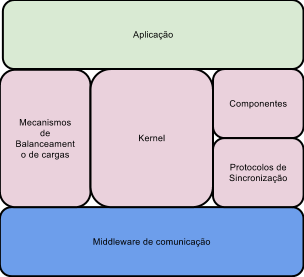
\includegraphics{arquitetura_macro.png}}
  \caption{Camadas da arquitetura do \textit{framework}.}
\label{fig:arquitetura_macro}
\end{figure}

Conforme descrito na seção~\ref{solucoes_existentes}, os mecanismos de troca de mensagens existentes não contemplam nativamente os requisitos que possibilitem tanto a troca de mensagem entre processos e sua migração e, ao mesmo tempo, opere de forma transparente quanto à referenciação de processos lógicos que migraram. Nos casos que mais se aproximam dos requesitos do sistema, os agentes móveis, há uma transparência na troca de mensagens até o momento em que um agente migra para um nó distinto do sistema. Ao se mover para um ambiente diferente do seu ambiente de origem, implementações de agentes móveis como \textit{Aglets} carecem de uma intervenção do usuário para que se refatore os valores dos endereços físicos dos objetos. O middleware aqui proposto visa resolver este problema, tornando a comunicação entre processos completamente transparente para o seu usuário.

\section{Organização deste documento}

Os capítulos seguintes tratam da descrição detalhada da arquitetura do projeto e de sua implementação. O capítulo quatro trata da arquitetura do \textit{middleware} de comunicação. O capítulo cinco traz detalhes da arquitetura do \textit{framework} de simulação.

No capítulo seis é demonstrado detalhes de implementação que o autor julga conveniente explicitar neste documento e  alguns exemplos de simulação utilizando o framework desenvolvido.

Por fim o capítulo sete traz as discussões sobre os resultados desse trabalho, tanto quanto conclusões e propostas para sua continuaidade em trabalhos futuros.

